%% History:
% Pavel Tvrdik (26.12.2004)
%  + initial version for PhD Report
%
% Daniel Sykora (27.01.2005)
%
% Michal Valenta (3.12.2008)
% rada zmen ve formatovani (diky M. Duškovi, J. Holubovi a J. Žďárkovi)
% sjednoceni zdrojoveho kodu pro anglickou, ceskou, bakalarskou a diplomovou praci

% One-page layout: (proof-)reading on display
%%%% \documentclass[11pt,oneside,a4paper]{book}
% Two-page layout: final printing
\documentclass[11pt,twoside,a4paper]{book}   
%=-=-=-=-=-=-=-=-=-=-=-=--=%
% The user of this template may find useful to have an alternative to these 
% officially suggested packages:
\usepackage[czech, english]{babel}
\usepackage[T1]{fontenc} % pouzije EC fonty 
% pripadne pisete-li cesky, pak lze zkusit take:
% \usepackage[OT1]{fontenc} 
\usepackage[utf8]{inputenc}
%=-=-=-=-=-=-=-=-=-=-=-=--=%
% In case of problems with PDF fonts, one may try to uncomment this line:
%\usepackage{lmodern}
%=-=-=-=-=-=-=-=-=-=-=-=--=%
%=-=-=-=-=-=-=-=-=-=-=-=--=%
% Depending on your particular TeX distribution and version of conversion tools 
% (dvips/dvipdf/ps2pdf), some (advanced | desperate) users may prefer to use 
% different settings.
% Please uncomment the following style and use your CSLaTeX (cslatex/pdfcslatex) 
% to process your work. Note however, this file is in UTF-8 and a conversion to 
% your native encoding may be required. Some settings below depend on babel 
% macros and should also be modified. See \selectlanguage \iflanguage.
%\usepackage{czech}  %%%%%\usepackage[T1]{czech} %%%%[IL2] [T1] [OT1]
%=-=-=-=-=-=-=-=-=-=-=-=--=%

%%%%%%%%%%%%%%%%%%%%%%%%%%%%%%%%%%%%%%%
% Styles required in your work follow %
%%%%%%%%%%%%%%%%%%%%%%%%%%%%%%%%%%%%%%%
\usepackage{graphicx}
%\usepackage{indentfirst} %1. odstavec jako v cestine.
\usepackage{zref-savepos}
\usepackage{k336_thesis_macros} % specialni makra pro formatovani DP a BP
 % muzete si vytvorit i sva vlastni v souboru k336_thesis_macros.sty
 % najdete  radu jednoduchych definic, ktere zde ani nejsou pouzity
 % napriklad: 
 % \newcommand{\bfig}{\begin{figure}\begin{center}}
 % \newcommand{\efig}{\end{center}\end{figure}}
 % umoznuje pouzit prikaz \bfig namisto \begin{figure}\begin{center} atd.

\makeatletter
% \zsaveposx is defined since 2011/12/05 v2.23 of zref-savepos
\@ifundefined{zsaveposx}{\let\zsaveposx\zsavepos}{}
\makeatother
\newcounter{hposcnt}
\renewcommand*{\thehposcnt}{hpos\number\value{hposcnt}}
\newcommand*{\SP}{% set position
  \stepcounter{hposcnt}%
  \zsaveposx{\thehposcnt s}%
}
\makeatletter
\newcommand*{\UP}{% use previous position
  \zsaveposx{\thehposcnt u}%
  \zref@refused{\thehposcnt s}%
  \zref@refused{\thehposcnt u}%
  \kern\zposx{\thehposcnt s}sp\relax
  \kern-\zposx{\thehposcnt u}sp\relax
}
\makeatother


%%%%%%%%%%%%%%%%%%%%%%%%%%%%%%%%%%%%%
% Zvolte jednu z moznosti 
% Choose one of the following options
%%%%%%%%%%%%%%%%%%%%%%%%%%%%%%%%%%%%%
\newcommand\TypeOfWork{Diplomová práce} \typeout{Diplomova prace}
% \newcommand\TypeOfWork{Master's Thesis}   \typeout{Master's Thesis} 
% \newcommand\TypeOfWork{Bakalářská práce}  \typeout{Bakalarska prace}
% \newcommand\TypeOfWork{Bachelor's Project}  \typeout{Bachelor's Project}


%%%%%%%%%%%%%%%%%%%%%%%%%%%%%%%%%%%%%
% Zvolte jednu z moznosti 
% Choose one of the following options
%%%%%%%%%%%%%%%%%%%%%%%%%%%%%%%%%%%%%
% nabidky jsou z: http://www.fel.cvut.cz/cz/education/bk/prehled.html

%\newcommand\StudProgram{Elektrotechnika a informatika, dobíhající, Bakalářský}
%\newcommand\StudProgram{Elektrotechnika a informatika, dobíhající, Magisterský}
% \newcommand\StudProgram{Elektrotechnika a informatika, strukturovaný, Bakalářský}
 \newcommand\StudProgram{Elektrotechnika a informatika, strukturovaný, Navazující magisterský}
% \newcommand\StudProgram{Softwarové technologie a management, Bakalářský}
% English study:
% \newcommand\StudProgram{Electrical Engineering and Information Technology}  % bachelor programe
% \newcommand\StudProgram{Electrical Engineering and Information Technology}  %master program


%%%%%%%%%%%%%%%%%%%%%%%%%%%%%%%%%%%%%
% Zvolte jednu z moznosti 
% Choose one of the following options
%%%%%%%%%%%%%%%%%%%%%%%%%%%%%%%%%%%%%
% nabidky jsou z: http://www.fel.cvut.cz/cz/education/bk/prehled.html

%\newcommand\StudBranch{Výpočetní technika}   % pro program EaI bak. (dobihajici i strukt.)
\newcommand\StudBranch{Výpočetní technika}   % pro prgoram EaI mag. (dobihajici i strukt.)
%\newcommand\StudBranch{Softwarové inženýrství}            %pro STM
%\newcommand\StudBranch{Web a multimedia}                  % pro STM
%\newcommand\StudBranch{Computer Engineering}              % bachelor programe
%\newcommand\StudBranch{Computer Science and Engineering}  % master programe


%%%%%%%%%%%%%%%%%%%%%%%%%%%%%%%%%%%%%%%%%%%%
% Vyplnte nazev prace, autora a vedouciho
% Set up Work Title, Author and Supervisor
%%%%%%%%%%%%%%%%%%%%%%%%%%%%%%%%%%%%%%%%%%%%

\newcommand\WorkTitle{Simulace inhibice zpětného vychytávání pomocí neuronové sítě typu KVAZI-$\omega$}
\newcommand\FirstandFamilyName{Bc. Cornelius Hron}
\newcommand\Supervisor{prof. Ing. Damián Zlo, CSc.}


% Pouzijete-li pdflatex, tak je prijemne, kdyz bude mit vase prace
% funkcni odkazy i v pdf formatu
\usepackage[
pdftitle={\WorkTitle},
pdfauthor={\FirstandFamilyName},
bookmarks=true,
colorlinks=true,
breaklinks=true,
urlcolor=red,
citecolor=blue,
linkcolor=blue,
unicode=true,
]
{hyperref}




\begin{document}

%%%%%%%%%%%%%%%%%%%%%%%%%%%%%%%%%%%%%
% Zvolte jednu z moznosti 
% Choose one of the following options
%%%%%%%%%%%%%%%%%%%%%%%%%%%%%%%%%%%%%
\selectlanguage{czech}
%\selectlanguage{english} 

% prikaz \typeout vypise vyse uvedena nastaveni v prikazovem okne
% pro pohodlne ladeni prace


\iflanguage{czech}{
	 \typeout{************************************************}
	 \typeout{Zvoleny jazyk: cestina}
	 \typeout{Typ prace: \TypeOfWork}
	 \typeout{Studijni program: \StudProgram}
	 \typeout{Obor: \StudBranch}
	 \typeout{Jmeno: \FirstandFamilyName}
	 \typeout{Nazev prace: \WorkTitle}
	 \typeout{Vedouci prace: \Supervisor}
	 \typeout{***************************************************}
	 \newcommand\Department{Katedra počítačů}
	 \newcommand\Faculty{Fakulta elektrotechnická}
	 \newcommand\University{České vysoké učení technické v Praze}
	 \newcommand\labelSupervisor{Vedoucí práce}
	 \newcommand\labelStudProgram{Studijní program}
	 \newcommand\labelStudBranch{Obor}
}{
	 \typeout{************************************************}
	 \typeout{Language: english}
	 \typeout{Type of Work: \TypeOfWork}
	 \typeout{Study Program: \StudProgram}
	 \typeout{Study Branch: \StudBranch}
	 \typeout{Author: \FirstandFamilyName}
	 \typeout{Title: \WorkTitle}
	 \typeout{Supervisor: \Supervisor}
	 \typeout{***************************************************}
	 \newcommand\Department{Department of Computer Science and Engineering}
	 \newcommand\Faculty{Faculty of Electrical Engineering}
	 \newcommand\University{Czech Technical University in Prague}
	 \newcommand\labelSupervisor{Supervisor}
	 \newcommand\labelStudProgram{Study Programme} 
	 \newcommand\labelStudBranch{Field of Study}
}




%%%%%%%%%%%%%%%%%%%%%%%%%%    Poznamky ke kompletaci prace
% Nasledujici pasaz uzavrenou v {} ve sve praci samozrejme 
% zakomentujte nebo odstrante. 
% Ve vysledne svazane praci bude nahrazena skutecnym 
% oficialnim zadanim vasi prace.
{
\pagenumbering{roman} \cleardoublepage \thispagestyle{empty}
\chapter*{Na tomto místě bude oficiální zadání vaší práce}
\begin{itemize}
\item Toto zadání je podepsané děkanem a vedoucím katedry,
\item musíte si ho vyzvednout na studiijním oddělení Katedry počítačů na Karlově náměstí,
\item v jedné odevzdané práci bude originál tohoto zadání (originál zůstává po obhajobě na katedře),
\item ve druhé bude na stejném místě neověřená kopie tohoto dokumentu (tato se vám vrátí po obhajobě).
\end{itemize}
\newpage
}

%%%%%%%%%%%%%%%%%%%%%%%%%%    Titulni stranka / Title page 

\coverpagestarts

%%%%%%%%%%%%%%%%%%%%%%%%%%%    Podekovani / Acknowledgements 

\acknowledgements
\noindent
Chtěl bych poděkovat vedoucímu své diplomové práce Ing. Ondřeji Mackovi za pomoc
s vypracovávánáním této práce. Dále bych chtěl poděkovat svým kolegům z týmu
Migdb, obzvláště Martinu Mazanci, kteří svými připomínkami napomáhali k zkvalitnění této práce a
zahlazení některých nepřesností. V neposlední řadě bych chtěl poděkovat
firmě CollectionsPro s.r.o, jež přišla s původní myšlenkou, která vedla k
vytvoření Migdb týmu.


%%%%%%%%%%%%%%%%%%%%%%%%%%%   Prohlaseni / Declaration 

\declaration{V~Praze dne 22.\,5.\,2014}
%\declaration{In Kořenovice nad Bečvárkou on May 15, 2008}


%%%%%%%%%%%%%%%%%%%%%%%%%%%%    Abstract 
 
\abstractpage
\noindent 
This work is concerned with specifying the contract and implement the transformation changes 
of the application model into changes of the database model. It also
deals with the automation of the derivation of the changes applied to one model
leading to another without loss or with minimal loss of stored data.

% Prace v cestine musi krome abstraktu v anglictine obsahovat i
% abstrakt v cestine.
\vglue60mm

\noindent{\Huge \textbf{Abstrakt}}
\vskip 2.75\baselineskip

\noindent
Tato práce se zabývá upřesněním kontraktu a realizací transformací změn
aplikačního modelu na změny modelu databázového. Dále se zabývá automatizací odvození změn vedoucích z
jednoho modelu k druhému bez ztráty či s minimální ztrátou uložených dat.
%Abstrakt práce by měl velmi stručně vystihovat její podstatu. Tedy čím se práce
% zabývá a co je jejím výsledkem/přínosem.

\noindent
%Očekávají se cca 1 -- 2 odstavce, maximálně půl stránky.

%%%%%%%%%%%%%%%%%%%%%%%%%%%%%%%%  Obsah / Table of Contents 

\tableofcontents


%%%%%%%%%%%%%%%%%%%%%%%%%%%%%%%  Seznam obrazku / List of Figures 

\listoffigures


%%%%%%%%%%%%%%%%%%%%%%%%%%%%%%%  Seznam tabulek / List of Tables

\listoftables


%**************************************************************

\mainbodystarts
% Odsazeni prvniho radku odstavce resi class book (neaplikuje se na prvni 
% odstavce kapitol, sekci, podsekci atd.) Viz usepackage{indentfirst}.
% Chcete-li selektivne zamezit odsazeni 1. radku nektereho odstavce,
% pouzijte prikaz \noindent.

%**************************************************************

% Pro snadnejsi praci s vetsimi texty je rozumne tyto rozdelit
% do samostatnych souboru nejlepe dle kapitol a tyto potom vkladat
% pomoci prikazu \include{jmeno_souboru.tex} nebo \include{jmeno_souboru}.
% Napr.:
% \input{1_uvod.tex}
% \input{2_teorie.tex}
% atd...

%*****************************************************************************
\chapter{Úvod}
\section{Motivace}

V průběhu poslední dekády je vyvíjeno více nového softwaru než kdy předtím a
současně je i stávající software stále více a častěji modifikován, ať už
je to zapříčiněno  existencí rozsáhlého legacy systému, špatného návrhu či
upravovánim funkcionality softwaru. Dá se předpokládat, že díky masivnímu
rozšíření informačních technologií, obzvláště mobilních tento trend nejenže bude
pokračovat, ale bude i dále na vzestupu.

Díky nutnosti zpracování a ukládání velkého množství dat se již od padesátých
let dvacátého století prosazovaly myšlenky vedoucí k vytvoření speciálních
systémů k těmto účelům určeným - tento software se v české odborné literatuře
nazývá systém řízení báze dat (SŘBD). 

Kvůli nutnosti modifikace, dokumentace a komunikace mezi vývojáři vznikají různé
typy modelů. Objektový model aplikace popisuje strukturu aplikace a je doplněn
modelem databázovým modelem popisujícím stav databáze. Aby byla aplikace
funkční, je nutné zajistit konzistenci mezi databázovým a aplikačním modelem.
Tato konzistence je zaručena automatickou transformací aplikačního modelu na
model databázový, což vývojářům softwaru šetří čas strávený vývojem softwaru.
Tento problém byl již vyřešen a jeho řešení bývá v literatuře nazýváno objektově
relační mapování(ORM). Dnešní implementace ORM jsou schopny nejen transformovat
aplikační model na model databázový, ale také vyjádřit změnu v struktuře
aplikace pomocí DDL SQL skriptů, které pozmění model databázový tak aby
odpovídal modelu aplikačnímu. Problém nastává, jakmile zahrneme do zachování
nejen strukturu dat, ale i samotná data. Změnit strukturu dat a zároveň
transformovat data tak, aby měla stejnou vyjadřovací schopnost jako původní
data(považujme změny aplikačního modelu jako smazání třídy, atributu apod za
změny zachovávající informaci).


\section{Projekt Migdb}

Tato dipomová práce byla napsána v rámci projektu Migdb. Zabývá se zkoumáním
změn aplikačního modelu, jejich popisem a rozpoznáváním změn vedoucích od
jednoho aplikačního modelu vedoucích k druhému. Dále pak dokončuje a upřesňuje
kontrakt takzvaných operací nad aplikačním modelem a popisuje jejich
transformaci na změny modelu databázového. Ne nepodstatnou částí je poté
vygenerování SQL příkazů spustitelných nad relační databází PostgreSQL.

V rámci Migdb byly v posledních letech vytvořeny již vytvořeny 4 bakalářské
práce členů Migdb. Jednalo se o práce mé osoby jež pojednávala o problematice
mapování aplikačního modelu na model databázový Jiřího Ježka, dále práce Petra
Taranta popisující databázového modelu a poslední práce pojednává o popisu
testování projektu.

Projekt Migdb byl započat v spolupráci se společností Collections Pro a byl
prezentován na konferenci Code Generation v Cambridge.

\section{Aplikační model}

Aplikační model zachycuje vztahy mezi jednotlivými objekty tvořícími
aplikaci. Ačkoliv byl tento model vytvořen již v raných fázích projektu Migdb a
byl často upravován, tak se charakter popisující objekty v aplikačním modelu
příliš nezměnil. Některé entity v modelu se zjednodušily,
již neexistují atributy tableName a columnName, které byly obsaženy v první
verzi modelu.

\subsection{Operace nad aplikačním modelem}
\subsubsection{Cíle při modelování operací}

V průběhu modelování operací nad aplikačním modelem jsme se snažili, aby tyto
operace byly jednoznačné(strojově zpracovatelné) v rámci daného kontextu, dále
vzhledem k nutnosti textového zápisu uživatelem o minimalističnost zápisu. Tyto
dva koncepty jdou obecně proti sobě, proto jsme došli k jistému jejich
kompromisu uživatelské jednoduchosti zápisu a jednoznačnosti.

\subsubsection{Seznam aplikačních operací}

Operace v aplikačním modelu se vyvíjeli parametricky, ale také se měnil jejich
seznam. Z operací v první verzi modelu byly odstraněny operace MoveProperty,
AddPrimitiveClass, SetOpposite a SetType. Operace AddPrimitive byla označena za
nadbytečnou, protože není cílem modifikace modelu změna seznamu primitivních tříd, který bývá
definován použitým programovacím jazykem a tudíž by měl tento seznam být v
vstupní generaci. V průběhu analýzy operace SetOpposite bylo zjištěno, že tato
operace má smysl na strukturální úrovni, ale není možné ji aplikovat na obecná
data, proto byla tato operace nahrazena dvojicí operací ChangeUniToBidir a
ChangeBiToUnidir, které plní nároky kladené na původní operaci a jsou
aplikovatelné na datové úrovni. Operace SetType byla prozkoumána, ale
nebyla exaktně popsána, nebylo nalezeno její mapování na operace v databázi ani
validační podmínky nutné k úspěšné aplikaci operace na aplikační model. Je
očekatelné, že by tato operace měla souviset s dědičnými hierarchiemi. Operace
jsou uvedeny v tabulkách \ref{tab:opsSeznam1} a \ref{tab:opsSeznam2}. Kromě regulérních 
operací, které může vytvořit uživatel jsou v tabulce \ref{tab:opsSeznam2} uvedeny operace 
DistributeProperty, MergeProperty a operace ExportProperty, které jsou používány jako pomocné 
v implementaci složitějších reduktivních a expanzivních operací a manipulují s Property v rámci 
dědičné struktury.


\begin{table}
\begin{center}
\begin{tabular}{| c|| p{5cm}|p {6cm}|}
\hline
\bfseries Název operace & \bfseries popis &
\bfseries parametry \\[2mm] 
\hline \hline
AddStandardClass & Operace vytvoří novou třídu a její id odvozené z názvu třídy
& name, isAbstract, inHeritanceType \\
\hline
RenameEntity & Operace změní název třídy na nový & name, newName\\
\hline
SetAbstract & Operace nastaví třídě atribut abstract na danou hodnotu & name,
isAbstract\\
\hline
RemoveEntity & Operace odstraní entitu (standardní třídu) z modelu & name\\
\hline
AddProperty & Operace vytvoří v dané třídě novou property & owningClassName,
name - jméno vytvořené property, typeName - typ vytvářené property, lowerBound - dolní mez property, 
upperBound - horní mez, isOrdered - isUnique\\
\hline
RenameProperty & Přejmenuje property & owningClassName, name, newName \\
\hline
RemoveProperty & Odstraní property z třídy & owningClassName, name \\
\hline
SetBounds & Nastaví horní a dolní hranici property & upperBound, lowerBound \\
\hline
SetOrdered & Nastaví property seřaditelnost & owningClassName, name, isOrdered
\\
\hline
SetUnique & Nastaví property unikátnost & owningClassName, name, isUnique \\
\hline
AddParent & Nastaví třídě předka a přesune překrývající atributy do rodičovské
třídy & className, parentClassName
\\
\hline
RemoveParent & Odstraní třídě rodičovskou třídu a rozdistribuje data z
rodičovské třídy do nově nezávislé třídy (původního potomka) & className \\
\hline
ExtractClass & Vytvoří novou třídu, kterou napojí na původní třídu, exportuje
do nově vzniklé třídy vyjmenované property & sourceClassName, extractClassName,
associationPropertyName, oppositePropertyName, propertyNames \\
\hline 
InlineClass & Přesune property a jejich data do cílové třídy s ohledem na
unidirectional asociaci & targetClassName, associationPropertyName,
extractPropertyNames\\
\hline
ChangeUniToBidir & Vytvoří zpětný link k property a nastaví správně data &
className, associationPropertyName, oppositePropertyName \\
\hline
ChangeBiToUnidir & Odstraní opoziční property & className,
associationPropertyName \\
\hline
\end{tabular}
\end{center}
\caption{Seznam operací část 1}
\label{tab:opsSeznam1}
\end{table}

\begin{table}
\begin{center}
\begin{tabular}{| c|| p{5cm}|p {6cm}|}
\hline
\bfseries Název operace & \bfseries popis &
\bfseries parametry \\[2mm] 
\hline \hline
CollapseHierarchy & Exportuje property z jedné třídy do jejího předka a třídy
spojí, upraví dědičné vazby & superClassName, subClassName, isIntoSub\\
\hline
ExtractSubClass & Vytvoří třídě nového potomka a přesune do něj vyjmenované
property & sourceClassName, extractedClassName, extractedPropertyNames\\
\hline
ExtractSuperClass & Vytvoří třídě nového předka a přesune do něj vyjmenované
property, pokud měla původní třída předka nastaví tohoto předka rodičem nově
vzniklé třídě & sourceClassesName, extractParentName, propertyNames \\
\hline
PullUpProperties & Exportuje property do rodičovské třídy & childClassName,
pulledPropertiesNames\\
\hline
PushDownProperties & Exportuje vyjmenované property do třídy potomka a přesune JEN data potomka &
childClassName, pushedPropertiesNames\\
\hline
ExportProperty(virtuální operace) & Exportuje property v rámci hierarchie a data do cílové třídy & exportedPropertyName, 
className
\hline
DistributeProperty(virtuální operace) & Zduplikuje strukturu dané property do cílové třídy a přesune data přiřazená 
této třídě & DistributedPropertyName, className
\hline
MergeProperty(virtuální operace) & Přesune data zdrojové property do cílové property a smaže strukturu původní property & 
mergedPropertyName, className
\hline
\end{tabular}
\end{center}
\caption{Seznam operací část 2}
\label{tab:opsSeznam2}
\end{table}

\subsubsection {Rozdělení aplikačních operací} 

Operace nad aplikačním modelem je možné dělit podle dvou kritérií - 1. nad jakým
typem entity pracují, 2. jaký je charakter/význam pro tito entity daná operace
má.

První kritérium dělí aplikační operace na operace pracující s třídami a operace
pracující pouze s properties daných tříd. Podle druhého kritéria je možné
rozdělit operace nad aplikačním modelem 5 skupin - konstruktivní, destruktivní,
expanzivní, reduktivní a modifikační operace. Konstruktivní operace jsou takové,
které po své aplikaci vytvoří 1 novou entitu v výsledném modelu, která nemá žádné 
vazby na jiné entity. Příkladem aditivní operace je
operace AddClass. Destruktivní operace je opak konstruktivní, v vstupním modelu
existuje entita a ta je aplikaci destruktivní operace odstraněna. Operace
expanzivní přídává do výstupního modelu jednu entitu, čímž se podobá operaci
konstruktivní, nicméně zároveň je vázána na jinou entitu stejného typu a
zmenšuje její obsah. Příkladem expanzivní operace je ExtractClass. Reduktivní
operace je inverzí k operaci expanzivní. Tato operace entitu z vstupního
modelu odstraní a zároveň entitě, která je pro operaci řídící změní obsah.
Příkladem této operace je InlineClass.\\

Rozdělení operací nad aplikačním modelem je jen formální, neprojevilo se změnou
hierarchické struktury operací. Struktura operací byla zjednodušena - již
neexistuje rozhlodatelná operace ComposedOperation, všechny operace jsou nyní
defakto atomické. Tato změna byla zapříčiněna neschopností rozložit některé
dekomponovatelné operace na operace atomické. Je zde nutné podotknout, že tento
rozklad je v nynější chvíli možný, ačkoliv si vyžádal neformální
obohacení aplikačního modelu o některé atomické operace jakými jsou
mergePropery, distributeProperty a exportProperty. Tyto operace v aplikačním
modelu neexistují, ale v rámci transformace ODBCHM jsou v metodách
použity/volány.\\

\subsubsection{Vlastnosti operací}

V literatuře mají operace některé specifické vlastnosti jako je
invertovatelnost a rozložitelnost. Je nutné říci, že operace zmiňované v
literatuře pracují jen se strukturou dat, nikoliv s daty samotnými a jsou
kontextově nezávislé - tyto operace jsou tvořeny téměř výlučně konstruktivními
a destruktivními operacemi. V projektu Migdb na druhé straně existují operace, 
které jsou kontextově závislé, což je uživatelskou přívětivostí
operací - jako zástupcem takové operace se dá uvést operace
AddParent(parentClass=B, childClass=A), která nezmiňuje všechny Property, které
se mají odstranit, ale dynamicky si je dopočítává v závislosti na daném
kontextu. Její inverzí je operace RemoveParent(childClass=A). Vzhledem k
minimalističnosti neexistuje k operaci RemoveParent(childClass=A) jednoznačná 
inverze bez daného konktextu.

Inverzi AddParent(sourceClass=A parentClass=B) získáme, pokud v
kontextu přidruženém modelu aplikaci RemoveParent má třída A předka B. Nicméně i
v takovém případě neplatí, že aplikace sekvence těchto dvou inverzních operací
na vstupní model M vygeneruje vždy původní model. Příkladem tohoto neočekávaného
chování je vstupní model Man(int age, String name), Person(int age, String name, String sureName).
Aplikace operace AddParent(Man, Person) odstraní přebytečné atributy v třídě man
a přidá rodiče této třídě, tj vznikne model : Man()->Person, Person(int age,
String name, String sureName). Nyní je aplikována operace RemoveParent(Person),
která sice získá z modelu jméno rodičovské třídy, ale nezíská seznam property,
které se distribuují do třídy Man. Operace byly navrženy tak, aby maximalizovali
objem zachovaných dat, proto operace RemoveParent distribuuje všechny
atributy třídy Person do třídy Man. Výsledný model je tedy: Man(int age, String
name, String sureName), Person(int age, String name, String sureName) a odlišuje
se od vstupního modelu o property sureName v třídě Man.

Stejná vlastnost platí pro dvojici ChangeUniToBidir a ChangeBiToUnidir, s
rozdílem, že se nejedná o automaticky získanou rodičovskou třídu, ale
opozitní property.

\section{ODBCHM operací}

Ačkoliv v průběhu projektu Migdb byla transformace operace z aplikačního modelu
na sadu operací databázových označována jako ORM operací, rozhodli jsme se
změnit název této transformace na Operation Database Change Mapping, kde dána
databázová změna reprezentuje sadu DDL, DML operací, které vzniknou pomocí
transformace. Ačkoliv na úrovni aplikační všechny operace fungují se všemi inheritanceTypy 
bylo nutné zjednodušit aplikační model tak, aby byla transformace ODBCHM implementovatelná, 
proto jsme v rámci týmu Migdb rozhodli o redukci počtu inheritanceTypů na jeden - nejvhodnější
typ je nejspíše joined, který je pravděpodobně nejpoužívanějším. Vzhledem k nedostatku času nebyla implementována myšlenka .q 
souborů, které kontrolují některé vlastnosti nejen modelu, ale i konkrétních dat, dále není mapováno omezení LB = 0, 
které by některé operace stížilo. Algoritmus ODBCHM si bere všechna data z aplikačního modelu, čímž je nezávislý na aplikaci 
databázových operací nad databázovým modelem, ale předává veškerou zodpovědnost za údržbu - tj vytvoření a odstranění omezení.
V tabulkách \ref{tab:odbchmSeznam1} a \ref{tab:odbchmSeznam1} nejsou uvedena vytváření a 
odstraňování unikátních constrainů pro unikátní či ordered kolekce primitivních a neprimitivních typů. 

V tabulkách 

\begin{table}
\begin{center}
\begin{tabular}{| c|| p{5cm}|p {6cm}|}
\hline
\bfseries Název operace & \bfseries podmínky validnosti &
\bfseries Rozklad na db operace \\[2mm] 
\hline \hline
AddStandardClass & Neexistuje třída s jménem nově vznikající
&  Vytvoří tabulku, id sloupec této tabulky a primární klíč\\
\hline
RenameEntity &  Existuje třída s původním jménem, neexistuje třída s novým jménem & Operace změní název tabulky 
na nový, odstraní a vytvoří PK s novým jménem\\
\hline
SetAbstract & Existuje třída s daným jménem & pro isAbstract = true maže data, která náleží pouze dané třídě\\
\hline
RemoveEntity & Existuje třída s daným jménem, neexistuje link na tuto třídu, třída neobsahuje žádné property, 
neexistuje pro tuto třídu žádný potomek & V Db je smazán primární klíč, property a tabulka\\
\hline
AddProperty & zadané bounds jsou validní, v hierarchii dědičnosti neexistuje koliyní property & 
operace přidá do cílové tabulky atribut pro primitivní property S UB = 1\\
\ & \ & operace přidá tabulku, datový sloupec, referenční sloupec a referenci na vlastnickou tabulku pro primitivní 
property s UB = > 1\\
\ & \ & operace přidá sloupec pro neprimitivní property S UB = 1 do vlastnické tabulky a referenci na tabulku typu\\
\ & \ & operace vytvoří vazební tabulku pro neprimitivní property s UB > 1, vloží do ní referenční sloupce na 
vlastnickou tabulku a tabulku typu, na které vytvoří cizí klíč\\
\hline
RenameProperty & Existuje přejmenovaná property v dané třídě, nexistuje property v dané třídy nového jména & pro danou property s 
UB = 1 a primitivním typem přejmenuje property v vlastnické tabulce\\
\ & \ & pro danou primitivní property s UB > 1 přejmenuje datový sloupec, FK na vlastníka kolekce a tabulku kolekce \\
\ & \ & pro danou associační property přejmenuje sloupec v vlastnické tabulce a cizí klíč referující tabulku typu\\
\ & \ & pro danou asociační property přejmenuje vazební tabulku s referenčními sloupci na vlastníka a typ asociace + cizí klíče \\
\hline
RemoveProperty & Musí exitovat vlastnická třída property a v ní odstraňovaná property & pro primitivní property S UB = 1 odstraní 
sloupec z dané tabulky\\
\ & \ & pro danou property primitivního typu s UB > 1 odstraní referenci na vlastnickou tabulku, sloupec z tabulky dané kolekce, 
datový sloupec a smaže kolekční tabulku \\
\ & \ & pro danou asociační property s UB = 1 odstraní referenci na tabulku vlastníka a referenční sloupec\\
\ & \ & pro danou asociační property s UB > 1 odstraní reference na vlastnickou tabulku a tabulku typu, datový 
sloupec a sloupec typu a smaže vazební tabulku \\
\hline
SetBounds & bounds musí být validní a musí existovat daná trída a property & NEIMPLEMENTOVÁNO \\
\hline
SetOrdered & musí existovat daná trída a property & pro nastavní = true přidá sloupec ordering, (měl by přenastavit data) a vytvoří 
unikátní constraint přes typový, referenční a orgering sloupec\\
\ & \ & pro nastavení = false sma6e ordering constraint a ordering column\\
\hline
SetUnique & Nastaví property unikátnost & owningClassName, name, isUnique \\
\hline
AddParent & Musí existovat rodičovská třída a třída potomka, třída potomka nesmí mít nastaveného rodiče & 
Aplikuje obraz operace MergeProperty na všechny kolizní property, přidá cizí klíč na rodičovskou třídu\\
\hline
RemoveParent & & musí existovat třída child a mít nastavenou rodičovskou třídu & aplikuje obraz operace 
DistrubuteProperty na všechny property rodičovské třídy, odstraní cizí klíč, smaže data třídy potomka z 
tabulky rodiče\\
\hline
ExtractClass & Vytvoří novou třídu, kterou napojí na původní třídu, exportuje
do nově vzniklé třídy vyjmenované property & sourceClassName, extractClassName,
associationPropertyName, oppositePropertyName, propertyNames \\
\hline 
InlineClass & Přesune property a jejich data do cílové třídy s ohledem na
unidirectional asociaci & targetClassName, associationPropertyName,
extractPropertyNames\\
\hline
ChangeUniToBidir & Vytvoří zpětný link k property a nastaví správně data &
className, associationPropertyName, oppositePropertyName \\
\hline
ChangeBiToUnidir & Odstraní opoziční property & className,
associationPropertyName \\
\hline
\end{tabular}
\end{center}
\caption{ODBCHM Seznam operací část 1}
\label{tab:odbchmSeznam1}
\end{table}

\begin{table}
\begin{center}
\begin{tabular}{| c|| p{5cm}|p {6cm}|}
\hline
\bfseries Název operace & \bfseries popis &
\bfseries parametry \\[2mm] 
\hline \hline
CollapseHierarchy & Exportuje property z jedné třídy do jejího předka a třídy
spojí, upraví dědičné vazby & superClassName, subClassName, isIntoSub\\
\hline
ExtractSubClass & Vytvoří třídě nového potomka a přesune do něj vyjmenované
property & sourceClassName, extractedClassName, extractedPropertyNames\\
\hline
ExtractSuperClass & Vytvoří třídě nového předka a přesune do něj vyjmenované
property, pokud měla původní třída předka nastaví tohoto předka rodičem nově
vzniklé třídě & sourceClassesName, extractParentName, propertyNames \\
\hline
PullUpProperties & Exportuje property do rodičovské třídy & childClassName,
pulledPropertiesNames\\
\hline
PushDownProperties & Exportuje vyjmenované property do třídy potomka a přesune JEN data potomka &
childClassName, pushedPropertiesNames\\
\hline
ExportProperty(virtuální operace) & Exportuje property v rámci hierarchie a data do cílové třídy & exportedPropertyName, 
className
\hline
DistributeProperty(virtuální operace) & Zduplikuje strukturu dané property do cílové třídy a přesune data přiřazená 
této třídě & DistributedPropertyName, className
\hline
MergeProperty(virtuální operace) & Přesune data zdrojové property do cílové property a smaže strukturu původní property & 
mergedPropertyName, className
\hline
\end{tabular}
\end{center}
\caption{ODBCHM Seznam operací část 2}
\label{tab:odbchmSeznam2}
\end{table}

\section{Modul Migdb}
Původně modul mapování operace fungoval podle následujícího schématu:


Pro \SP každou vstupní operaci AOp\\
	\UP 1. validace AOp \\
    \UP 2. aplikace AOp na vstupní model \\
    \UP 3. Rozklad operace AOp na seznam db operací \\
    \UP 4. Pro každou\SP operaci DbOp rozkladu:\\ 
           \UP a) validace operace DbOp\\
           \UP b) aplikace operace DbOp
Generování SQL z seznamu DB OP
\\

Tento přístup narazil na některé problematické případy v průběhu testování
aplikace výsledných SQL nad daty v databázi. Z tohoto důvodu a z důvodu
přehlednější implementace bylo základní schéma modulu pozměneno a byl přidán
koncept mirroredOperations.

Představme si, že uživatel potřebuje aplikovat operaci ExtractClass(A, B,
props), A je třída, z které se extrahuje, B je nově vzniklá třída, do které se
budou přesouvat property z kolekce props a jejich data.

Tato oper\SP ace pracuje nad aplikačním modelem následovně: \\
         \UP Vytvoří třídu B\\
 		 \UP Vytvoří v třídě A referenční property, která bude mít typ B\\
 	     \UP Pro každou property z kolekce props aplikuje operaci MoveProp
 	     - vytvoří v třídě B Property, přesune data do nově vzniklé property,
 	     smaže ji z původní třídy A

Krok 1 se v databázi projeví standardně. V kroku 2. je v databázi kromě
vytvoření sloupce nutné vygenerovat data v nově vzniklé a referencovat je
v tabulce kdy není možné oddělit v ODBCH krok 2, vytvoření referenční Property.
V databázi je nutné vytvořit sloupec, nicméně tento sloupec musí obsahovat 

\subsection{Diff elementy}

 Kvůli nutnosti rozpoznávat operace vznikly v aplikačním modelu nové
 elementy. Kořenovým elementem diff modelu je Diff element. Tento element
 obsahuje kolekce elementů classpairs typů ClassPair, propertyPairs
 typu PropertyPair, a dále pak addedClasses a removedClasses typu DiffClass a
 addedProperties a removedProperties typu DiffProperty. Element ClassPair
 shlukuje zpárované zdrojové (source) a obrazové (reflection) třídy, dále pak
 referenci owningDiff na Diff element, v kterém jsou obsaženy a která je
 důležitá pro implementaci algoritmu a v neposlední řadě underlyingPairs -
 shodné páry Properties typu EqualPropertyPair, které jsou detekované danou
 operací. Podobně jako operace jsou i páry rozděleny do rodin ConstructiveClassPair,
 DestructiveClassPair a ModifyingClassPair, ale aby bylo možné rozpoznat specifický 
 pár závislý na jiném páru, byla přidána třída ReplacingClassPair - nahrazující pár,
 který se používá jako pivot pro hledání konstruktivních, destruktivních a 
 modifikačních párů. Od elementu ReplacingClassPair dědí elementy EqualClassPair 
 - třída, která si uchovala jméno z původního modelu a element ReplacingClassPair - 
 reprezentující třídu, která si neuchovala jméno, ale má změněný název. Podmínky 
 získávání konkrétních typů párů a jejich pořadí specifikuje konkrétní rozpoznávací 
 algoritmus.
 
 Projevem subtraktivních a aditivních operací jsou elementy DiffClass a
 DiffProperty, které zaobalují třídy a property tak, aby bylo možné referencovat
 na jiný objekt než element Structure. Oproti jednodušším operacím aditivním a
 subtraktivním jsou operace destruktivní, konstruktivní a modifikační v Diff
 modelu zobrazeny do elementů ConstructiveClassPair, DestructiveClassPair a
 ModifyingClassPair. 

\section{Rozpoznávání operací}

Algoritmem pro rozpoznávání operací nazveme každý algoritmus, který nám pro
každý vstupní model A a cílový model B najde uspořádaný seznam operací, jejichž
postupná aplikace transformuje model A do modelu B. Tento algoritmus nemusí být
deterministický.

Jedním z zajímavých faktů je poznatek, že seznam operací nemusí být jednoznačný
a to i u jednoduchých změn. Pokud aplikujeme sekvenci operaci Inline A, B + 
Rename B ->C na model X dostaneme stejný výstup jako aplikací operací Inline B,
A + Rename A->C, ještě zajímavějším poznatkem je, že nejsme schopni rozeznat
rozdíl mezi aplikací sekvence operací Rename A, C + Inline C, B.

Samostatným tématem je pořadí operací a jeho permutace. Je zřejmé, že pořadí v
seznamu operací operujících nad jinými elementy bude možné libovolně prohazovat.
Také je samozřejmé, že seznam subtraktivních operací je také možné libovolně
zpermutovat. Stejně tak seznam aditivních operací. Obecný princip seřazení kolekce 
operací není znám.

\section{Obecné principy model matching}
Jak je diskutováno v 19 a Different Models for Model Matching:
An analysis of approaches to support model differencing existuje několik
požadavků na algoritmus řešící problém model matching. Tyto požadavky zahrnují
přesnost, vysokou míru abstrakce na které je porovnávání provedeno, nezávislost
na konkrétních nástrojích, doménách a jazycích (přelož independence from
particular tools), použitelnost(efficiency) a minimální nutnost adaptace
algoritmus pro daný problém. Tyto požadavky jdou proti sobě a je nutné
preferovat některé na úkor jiných, proto není možné označit za nejlepší, ale je
nutné vybrat si správný algoritmus v závislosti na řešeném problému.

Nejtriviálnější implementovatelný algoritmus by mohl smazat zdrojový model
pomocí destruktivních operací a následně vytvořit výsledný model pomocí operací
konstruktivních, připadně poupravit atributy jednotlivých elementů pomocí
operací modifikačních. Argumentem proti použití takového algoritmu je smazání jakýchkoliv dat, které v
původní databázi byla a dobré si uvědomit, že funkci vytvoření DB modelu zvládá
ORM mapování integrované do většiny současných IDE.

 V literatuře (Different Models for Model Matching:
An analysis of approaches to support model differencing) byly popsány algoritmy
pro mapování shodných entit modelů (ModelMatching) a algoritmy pro získávání rozdílu modelů (Model Diff).
 Principem těchto modelů je párování elementů vstupního modelu s elementy z
 modelu cílového. Existují 4 obecné skupiny dělení matching algoritmů. 1
 párování podle statického identifikátoru, 2. signature based matching, 3.
 similarity based matching a custom language specific matching.
 
 Párování podle statického identifikátoru páruje elementy podle perzistentního
 identifikátoru, který je přiřazen každé entitě v době jejího vzniku, je
 neměnný a unikátní. Nejzákladnějším principem model matchingu je tedy párování
 entit na základě shodnosti jejich identifikátorů. Tento princip má výhody
 jednoduchosti implementace a rychlosti. Tento algoritmus není použitelný pro
 modely vytvořené nezávisle jeden na druhém či u technologií nepodporujících
 maintenance unikátních identifikátorů.
 
 Algoritmus signature based matching byl navržen kvůli limitaci párování podle
 statického identifikátoru, tento algoritmus je založen na dynamickém vypočtení
 nestatické signatury jednotlivých features pomocí uživatelem definovaných
 funkcí specifikovaných pomocí nějakého dotazovacího jazyka. Tento princip tedy
 může být použit pro modely vzniklé nezávisle na sobě. Nevýhodou je potom
 nutnost specifikovat query, které dopočítají signaturu.
 
 Algoritmus Similarity based matching používá podobně jako signature based
 matching podobnost features jednotlivých elementů, kterou agreguje do skalární hodnoty.
 Tento princip se řadí mezi podtyp attribute graph matchingu. Každá feature
 modelu může mít jinou váhu pro porovnávání, napřiklad u podobnosti tříd má
 jméno vyšší důležitost nežli abstractnost dané třídy.  Tento algoritmus musí
 být typicky doplněn o konfiguraci vah jednotlivých features elementů, kterou
 většinou píše vývojář. Zástupcem tohoto principu je framework EMF Compare, 
 který je doplněn o defaultní konfiguraci vah. Výhodami je větší přesnost,
 nevýhodou je potom TRIAL ERROR metoda získávání vhodné konfigurace vah.
 
 Algoritmy v kategorii Custom language specific matching jsou vytvořené
 přímo k využití daného modelovacího jazyka. Hlavní výhodou je, že
 algoritmus na dané doméně může začlenit do metody similarity based matchingu
 sémantické detaily, což vede k přesnějším výsledkům a redukuje prohledávaný 
stavový prostor. Jako příklad je uváděn jazyk UMLDiff, který při porovnávání
dvou UML modelů může využít faktu, že dvě třídy nebo dva datové typy
stejného jména tvoří po všech praktických stránkách pár(match). Nicméně výhoda
začlenění sémantických detailů konkrétní domény je vykoupeno vysokou cenou -
všechny ostatní kategorie algoritmů potřebují minimální neb téměř žádné úpravy
od vývojáře, pro tuto kategorii vývojáře musí napsat celý matchovací algoritmus
sám.

\subsection{Graph matching}
 Problém model matching je podproblémem generičtějšího tasku graph matching,
 který studuje http://www.sc.ehu.es/acwbecae/ikerkuntza/these/Ch2.pdf a
 rozděluje a popisuje algoritmy pro graph matching. Problém je definován na
 obecné struktuře Graf, což je uspořádaná dvojice G = (V, E), kde G je množina
 uzlů a E je množina hran grafu, přičemž $E \subset V \times V$. Grafy mohou být
 orientované či neorientované, mohou mít vícenásobné hrany.
 
 Každý graf může přidávat informace do své struktury pomocí labelu (popisku
 nebo číslu) do hran a vrcholů, pokud je nutné přidat více informací, je možné
 přidat do hran a/nebo vrcholů atributy, potom hovoříme o vertex-atributed
 grafech a edge atributed grafech, případně attributed grafech. V některé
 literatuře jsou attributed grafy označovány jako labeled grafy. Graph
 matching je aplikován v mnoho oborů jako je počítačové vidění, analýza
 scény(scene analysis), chemie a molekulární biologie. V těchto oborech musí být
 vzorce nalezeny v daných datech. 
  
 Problém graph matchingu dvou grafů $G_P$ (grafu patternu) a $G_M$ (grafu
 modelu), přičemž se dělí podle převzatého obrázku \ref{fig:graph_matching} na matching nalezení přesné shody vzorku v hledaném
 grafu či matching hledání podobnosti grafu vzorku v hledaném grafu. 
 
 Matching hledání přesné shody je definován následně: Mějme grafy $G_P = (V_P ,
 E_P)$ a $G_M = (V_M, E_M)$, přičemž $\| V_M\| = \| V_P\|$, úkolem je potom
 najít takové prosté zobrazení  $f: V_D \rightarrow V_M$, takové, že $(u, v) \in
 E_P$ iff $(f(u), f(v)) \in E_M$. Pokud takové mapování existuje, nazveme ho
 exact graph matchingem(matching přesné shody). \\
 
 Termín Inexact matching aplikovaný na některé problémy týkající se shodnosti grafů vyjadřuje/znamená, že není možné nalézt 
 izomorfismus mezi dvěma grafy, aby byly matched (shodné?). To je stav, kdy oba grafy mají jiný počet vrcholů. Takže v těchto 
 případech není očekávatelné hledání izomorfismu dvou grafů, ale v hledání největší možné shody mezi nimi (best matching). 
 Toto vede k třídě problémů známé jako inexact graph matching. V takovém případě hledáme nebijektivní korespondenci (přiřazení)
 mezi pattern grafem a model grafem. V následujícím textu předpokládejme
 $\|V_P\| < \|V_M\|$. Inexact matching je používán v oborech kartografie,
 rozpoznávání znaků a medicíně. Nejlepší korespondence graph matching problému je definována jako optimum nějaké objective function, ktérá měří podobnost mezi matchovanými uzly a hranami. Tato funkce je nazvána fitness funkcí, případně energy function.

 Formálně je tedy inexact matching definován takto: mějme dva grafy, $G_M a G_P$ přičemž $\| V_M \| < \| V_D\|$ a cílem je nalezení mapování
 $f' : V_D  \rightarrow V_M že (u, v) \in E_P$ iff $(f(u), f(v)) \in E_M$.\\
 
 Podtypem těchto úloh jsou problémy subgraph matching a subgraph izomorfizmu.
 
 Složitost uváděných problémů uvádí autor u Exact graph matchingu jako P až NP kompletní, přičemž že u problémů této kategorie nebyla dokázána nejvyšší složitost 
 NP complete. Pro složitost problémů u subgraph isomorphismu byla dokázáno, že patří do třídy NP complete. Pro složitost nepřesného graph matchingu bylo dokázáno, 
 že patří do třídy NP-complete. 
 
 
 
 \begin{figure}[ht]
\begin{center}
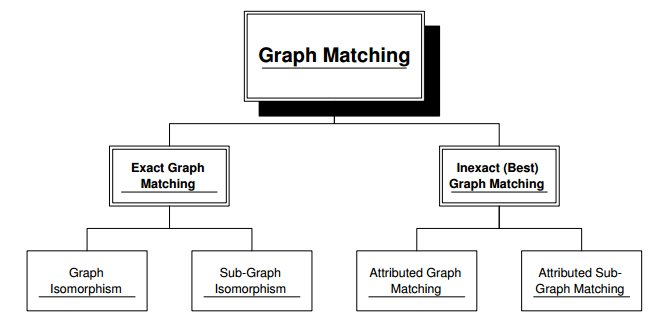
\includegraphics[width=15cm]{figures/graph_matching.jpg}
\caption{Typy graph matchingu}
\label{fig:graph_matching}
\end{center}
\end{figure}
 
 
 \section{Vytvořený algoritmus rozpoznávání operací}
 
 \subsection{Návrh ze studia článků}
 
 Vzhledem k obecné použitelnosti algoritmů pro graph matching nebyly tyto
 algoritmy shledány za vhodné k použití pro problém hledání sady
 aplikačních operací. První 3 popsané algoritmy model matchingu ( 1
 párování podle statického identifikátoru, 2. signature based matching, 3.
 similarity based matching) nejsou taktéž vhodné k použití z důdodu, že k rozpoznání popsaných
 expanzivních a reduktivních operací je nutné rozpoznat 2 třídy, které se mapují na jednu třídu pro reduktivní 
 operace a naopak jednu operaci, která se mapuje na 2 třídy. Problém rozpoznávání operací je tudíž nadskupinou problému 
 model matchingu, protože matching páruje 1 ku jedné, ale ná na algoritmus řešící rozpoznávání operací musí řešit 
 matching M entit ku N entitám. 
 
 Zmiňované algoritmy mě inspirovaly k vytvoření Custom language specific matching algoritmu pro tento problém, který si 
 z zmiňovaných algoritmů bere hlavně poznámku u UMLDiffu - ze všech praktických důvodů považujeme třídy se stejným jménem 
 jako matchující.

 \subsection{Implementace}
 Vzniklo několik implementací párovacích algoritmů. První a nejjednodušší
 používá párování tříd podle jména, následné rozdíly řeší rozpoznáním
 konstruktivních a destruktivnívh, případně některých operací modifikačních, ať
 už tyto operace pracovali s třídami nebo s property.
 
 Složitější implementace algoritmu bylo páruje stejně jako jednodušší v
 první fázi shodné elementy - modely se mění, ale některé třídy jsou zachovány.
Shodné elementy potom tvoří jakési pilíře pro operace konstruktivní a
destruktivní, které se vážou na rozpoznané páry. Závislost rozpoznání

Algoritmus rozpoznávání operací byl napsán se snahou o zachovávání co největšího
množství dat. Ačkoliv triviální algoritmus pro přechod z modelu A k modelu B by
mohl pomocí subtraktivních operací zničit model A a následně složit model B
pomocí aditivních operací je zřejmé, že tento algoritmus neuchová žádná data.
Proto byly zavedeny Konstruktivní a destruktivní operace. 

\section{alternativní algoritmus}

V ranné fázi byl napsán prototyp jiného rozpoznávacího algoritmu, který se snaží 
minimalizovat vzdálenost současného modelu od modelu cílového pomocí rozpoznáná 
operací a aplikace operací. Výhodou tohoto přístupu je nalezení více alternativních 
cest, nevýhodou je potom velikost stavového prostoru. Algoritmus prochází těmito fázemi:

Spočítání vzdálenosti vstupního modelu od modelu cílového
Nastavení nalezeného maxima na nula
Pro každou operaci O
     zjištění, jestli má operace vhodné kandidáty na parametr
     nalezení nejvhodnějších parametrů operace



% *****************************************************************************
\chapter{Popis problému, specifikace cíle}
Tato diplomová práce si klade za cíl dokončit vývoj na projektu Migdb. Tj
doimplementovat a otestovat ORM transformace vzniklé v předešlých fázích
projektu, upravit a otestovat generátor SQL, případně upravit aplikační a
databázový metamodel.

Dalším cílem, který jsem si před vypracováním diplomové práce stanovil bylo
vytvoření a zdokumentování algoritmu generující z dvou vstupních modelů
sekvenci operací, jejichž aplikací se model zdrojový transformuje na model
koncový.


\chapter{Ukázka zdrojového kódu práce}

%\begin{itemize}
%\item Popis řešeného problému, vymezení cílů DP/BP a požadavků na
% implementovaný systém.
%\item Popis struktury DP/BP ve vztahu k vytyčeným cílům.
%\item Rešeršní zpracování existujících implementací, pokud jsou známy.
%\end{itemize}

%*****************************************************************************
%\chapter{UML diagramy}
%\textbf{\large Tato příloha není povinná a zřejmě se neobjeví v každé práci.
% Máte-li ale větší množství podobných diagramů popisujících systém, není nutné všechny umísťovat do hlavního textu, zvláště pokud by to snižovalo jeho čitelnost.}

%*****************************************************************************
%\chapter{Instalační a uživatelská příručka}
%\textbf{\large Tato příloha velmi žádoucí zejména u softwarových
% implementačních prací.}

%*****************************************************************************
\chapter{Obsah přiloženého CD}
%\textbf{\large Tato příloha je povinná pro každou práci. Každá práce musí totiž
% obsahovat přiložené CD. Viz dále.}

%Může vypadat například takto. Váš seznam samozřejmě bude odpovídat typu vaší
%práce. (viz \cite{infodp}):

\begin{figure}[h]
\begin{center}
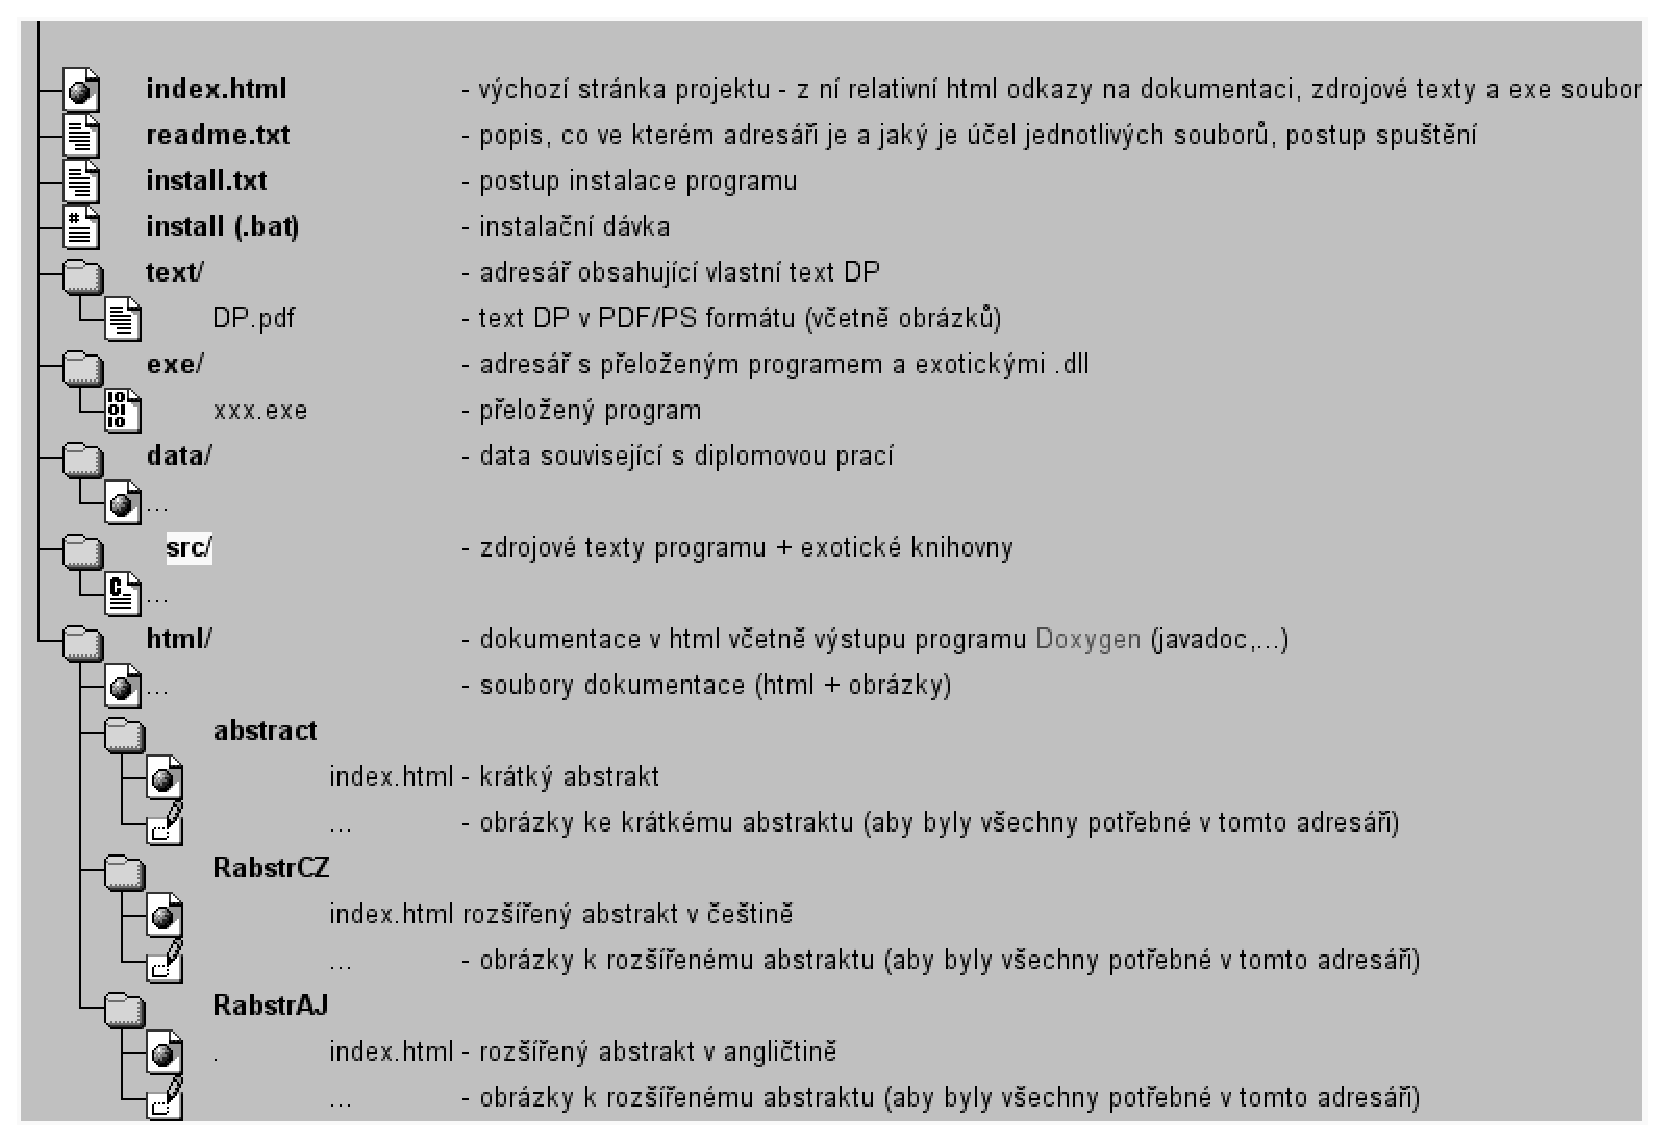
\includegraphics[width=14cm]{figures/seznamcd}
\caption{Seznam přiloženého CD}
\label{fig:seznamcd}
\end{center}
\end{figure}

\chapter{Závěr}
Ačkoliv se mi nepodařilo dokončit tuto diplomovou práci v termínu, dokončil jsem
implementační(viz ukázka kódu) a testovací části projektu, které jsem nestihl
zdokumentovat. Proto bych byl rád, kdybych mohl věnovat následující půlrok
přepracování textu diplomové práce.


\section{Odkazy v textu}
\subsection{Odkazy na literaturu}
Jsou realizovány příkazem \verb|\cite{odkaz}|. 

Seznam literatury je dobré zapsat do samostatného souboru a ten pak zpracovat programem bibtex (viz soubor \verb|reference.bib|). Zdrojový soubor pro \verb|bibtex| vypadá například takto:
\begin{verbatim}
@Article{Chen01,
  author  = "Yong-Sheng Chen and Yi-Ping Hung and Chiou-Shann Fuh",
  title   = "Fast Block Matching Algorithm Based on 
             the Winner-Update Strategy",
  journal = "IEEE Transactions On Image Processing",
  pages   = "1212--1222",
  volume  =  10,
  number  =   8,
  year    = 2001,
}

@Misc{latexdocweb,
  author  = "",
  title   = "{\LaTeX} --- online manuál",
  note    = "\verb|http://www.cstug.cz/latex/lm/frames.html|",
  year    = "",
}
...
\end{verbatim}

%11.12.2008, 3.5.2009
\textbf{Pozor:} Sazba názvů odkazů je dána Bib\TeX{} stylem\\ (\verb|\bibliographystyle{abbrv}|). 
%Budete-li používat české prostředí (\verb|\usepackage[czech]{babel}|), 
Bib\TeX{} tedy obvykle vysází velké pouze počáteční písmeno z názvu zdroje, 
ostatní písmena zůstanou malá bez ohledu na to, jak je napíšete. 
Přesněji řečeno, styl může zvolit pro každý typ publikace jiné konverze. 
Pro časopisecké články třeba výše uvedené, jiné pro monografie (u nich často bývá 
naopak velikost písmen zachována).

Pokud chcete Bib\TeX u napovědět, která písmena nechat bez konverzí 
(viz \texttt{title = "\{$\backslash$LaTeX\} -{}-{}- online manuál"} 
v~předchozím příkladu), je nutné příslušné písmeno (zde celé makro) uzavřít 
do složených závorek. Pro přehlednost je proto vhodné celé parametry 
uzavírat do uvozovek (\texttt{author = "\dots"}), nikoliv do složených závorek.

Odkazy na literaturu ve zdrojovém textu se pak zapisují:
\begin{verbatim}
Podívejte se na \cite{Chen01}, 
další detaily najdete na \cite{latexdocweb}
\end{verbatim}

Vazbu mezi soubory \verb|*.tex| a \verb|*.bib| zajistíte příkazem 
\verb|\bibliography{}| v souboru \verb|*.tex|.  V našem případě tedy zdrojový 
dokument \verb|thesis.tex| obsahuje příkaz\\
\verb|\bibliography{reference}|.

Zpracování zdrojového textu s odkazy se provede postupným voláním programů\\
\verb|pdflatex <soubor>| (případně \verb|latex <soubor>|), \verb|bibtex <soubor>| 
a opět\\ \verb|pdflatex <soubor>|.\footnote{První volání \texttt{pdflatex} 
vytvoří soubor s~koncovkou \texttt{*.aux}, který je vstupem pro program 
\texttt{bibtex}, pak je potřeba znovu zavolat program \texttt{pdflatex} 
(\texttt{latex}), který tentokrát zpracuje soubory s příponami \texttt{.aux} a 
\texttt{.tex}. 
Informaci o případných nevyřešených odkazech (cross-reference) vidíte přímo při 
zpracovávání zdrojového souboru příkazem \texttt{pdflatex}. Program \texttt{pdflatex} 
(\texttt{latex}) lze volat vícekrát, pokud stále vidíte nevyřešené závislosti.}


Níže uvedený příklad je převzat z dříve existujících pokynů studentům, kteří 
dělají svou diplomovou nebo bakalářskou práci v~Grafické skupině.\footnote{Několikrát 
jsem byl upozorněn, že web s těmito pokyny byl zrušen, proto jej zde přímo necituji. 
Nicméně příklad sám o sobě dokumentuje obecně přijímaný konsensus ohledně citací 
v~bakalářských a diplomových pracích na KP.} Zde se praví:
\begin{small}
\begin{verbatim}
...
j) Seznam literatury a dalších použitých pramenů, odkazy na WWW stránky, ...
 Pozor na to, že na veškeré uvedené prameny se musíte v textu práce 
 odkazovat -- [1]. 
Pramen, na který neodkazujete, vypadá, že jste ho vlastně nepotřebovali 
a je uveden jen do počtu. Příklad citace knihy [1], článku v časopise [2], 
stati ve sborníku [3] a html odkazu [4]: 
[1] J. Žára, B. Beneš;, and P. Felkel. 
     Moderní počítačová grafika. Computer Press s.r.o, Brno, 1 edition, 1998. 
     (in Czech). 
[2] P. Slavík. Grammars and Rewriting Systems as Models for Graphical User 
     Interfaces. Cognitive Systems, 4(4--3):381--399, 1997. 
[3] M. Haindl, Š. Kment, and P. Slavík. Virtual Information Systems. 
     In WSCG'2000 -- Short communication papers, pages 22--27, Pilsen, 2000. 
     University of West Bohemia. 
[4] Knihovna grafické skupiny katedry počítačů: 
     http://www.cgg.cvut.cz/Bib/library/ 
\end{verbatim}
\end{small}
\ldots{} abychom výše citované odkazy skutečně našli v (automaticky generovaném) seznamu literatury tohoto textu, musíme je nyní alespoň jednou citovat: Kniha \cite{kniha}, článek v~časopisu \cite{clanek}, příspěvek na konferenci \cite{sbornik}, www odkaz \cite{www}.

\subsection{Odkazy na obrázky, tabulky a kapitoly}
\begin{itemize}
\item Označení místa v textu, na které chcete později čtenáře práce odkázat, se provede příkazem \verb|\label{navesti}|. Lze použít v prostředích \verb|figure| a  \verb|table|, ale též za názvem kapitoly nebo podkapitoly.
\item Na návěští se odkážeme příkazem \verb|\ref{navesti}| nebo \verb|\pageref{navesti}|.
\end{itemize}

\section{Rovnice, centrovaná, číslovaná matematika}
Jednoduchý matematický výraz zapsaný přímo do textu se vysází pomocí prostředí \verb|math|, resp. zkrácený zápis pomocí uzavření textu rovnice mezi znaky \verb|$|.

Kód \verb|$ S = \pi * r^2 $| bude vysázen takto: $ S = \pi * r^2 $.

Pokud chcete nečíslované rovnice, ale umístěné centrovaně na samostatné řádky, pak lze použít prostředí \verb|displaymath|, resp. zkrácený zápis pomocí uzavření textu rovnice mezi znaky \verb|$$|. Zdrojový kód: 
\begin{verb}
|$$ S = \pi * r^2 $$|
\end{verb}
bude pak vysázen takto:
$$ S = \pi * r^2 $$

Chcete-li mít rovnice číslované, je třeba použít prostředí \verb|eqation|. Kód:
\begin{verbatim}
\begin{equation}
  S = \pi * r^2
\end{equation}

\begin{equation}
  V = \pi * r^3
\end{equation}
\end{verbatim}
je potom vysázen takto:
\begin{equation}
  S = \pi * r^2
\end{equation}

\begin{equation}
  V = \pi * r^3
\end{equation}

\section{Kódy programu}
Chceme-li vysázet například část zdrojového kódu programu (bez formátování), hodí se prostředí \verb|verbatim|: 
\begin{verbatim}
         (* nickname2 *)
Lego> Refine in1
             (do_reg (nickname1 h));
Refine by  in1 (do_reg (nickname1 h))
   ?4 : pcdata
   ?5 : pcdata
          (* surname2 *)
Lego> Refine surname1 h;
Refine by  surname1 h
   ?5 : pcdata
          (* email2 *)
Lego> Refine undo_reg (email1 h);
Refine by  undo_reg (email1 h)
*** QED ***
\end{verbatim}

\section{Další poznámky}
\subsection{České uvozovky}
V souboru \verb|k336_thesis_macros.tex| je příkaz \verb|\uv{}| pro sázení českých uvozovek. \uv{Text uzavřený do českých uvozovek.}

% JZ: 3.5.2009 \chapter z book zajistí automaticky
%\subsection{Začátky kapitol na liché stránky}
%Ve výsledném textu je dobré, když každá kapitola začíná na liché stránce. Tedy použijte:
%\begin{verbatim}
%  \cleardoublepage\include{1_uvod}
%  \cleardoublepage\include{2_teorie}
%   atd.\ldots{}
%\end{verbatim}

%*****************************************************************************
\chapter{Seznam použitých zkratek}

\begin{description}
\item[IDE] Integrated Development Environment
\item[ORM] Object-relational mapping
\item[EMF] Eclipse modeling framework
\end{description}
\vdots

%*****************************************************************************
\chapter{UML diagramy}
\textbf{\large Tato příloha není povinná a zřejmě se neobjeví v každé práci. Máte-li ale větší množství podobných diagramů popisujících systém, není nutné všechny umísťovat do hlavního textu, zvláště pokud by to snižovalo jeho čitelnost.}

%*****************************************************************************
\chapter{Instalační a uživatelská příručka}
\textbf{\large Tato příloha velmi žádoucí zejména u softwarových implementačních prací.}

%*****************************************************************************
\chapter{Obsah přiloženého CD}
\textbf{\large Tato příloha je povinná pro každou práci. Každá práce musí totiž obsahovat přiložené CD. Viz dále.}

Může vypadat například takto. Váš seznam samozřejmě bude odpovídat typu vaší práce. (viz \cite{infodp}):

\begin{figure}[h]
\begin{center}
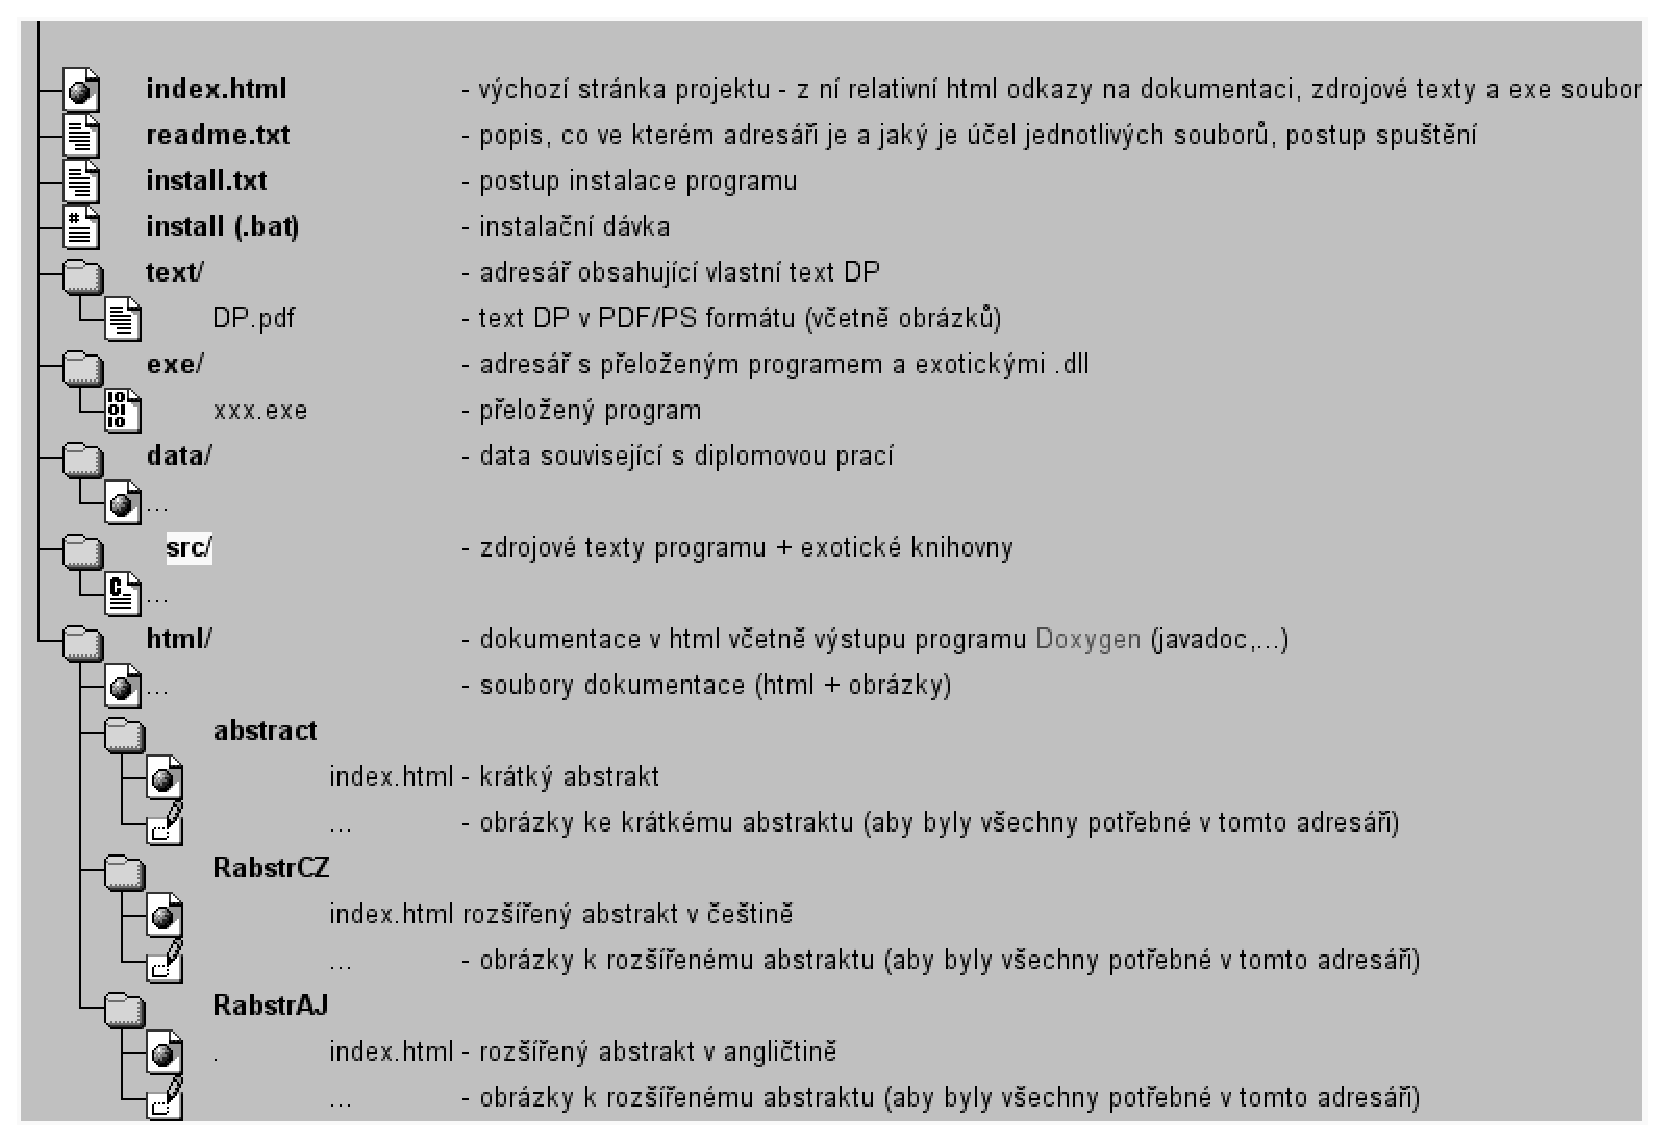
\includegraphics[width=14cm]{figures/seznamcd}
\caption{Seznam přiloženého CD --- příklad}
\label{fig:seznamcd}
\end{center}
\end{figure}

Na GNU/Linuxu si strukturu přiloženého CD můžete snadno vyrobit příkazem:\\ 
\verb|$ tree . >tree.txt|\\
Ve vzniklém souboru pak stačí pouze doplnit komentáře.

Z \textbf{README.TXT} (případne index.html apod.)  musí být rovněž zřejmé, jak programy instalovat, spouštět a jaké požadavky mají tyto programy na hardware.

Adresář \textbf{text}  musí obsahovat soubor s vlastním textem práce v PDF nebo PS formátu, který bude později použit pro prezentaci diplomové práce na WWW.

\end{document}
